% This must be in the first 5 lines to tell arXiv to use pdfLaTeX, which is strongly recommended.
\pdfoutput=1
% In particular, the hyperref package requires pdfLaTeX in order to break URLs across lines.

\documentclass[11pt]{article}
\usepackage{amsmath, adjustbox}
% Remove the "review" option to generate the final version.
\usepackage{EMNLP2022}

% Standard package includes
\usepackage{times}
\usepackage{latexsym}
\usepackage[normalem]{ulem}
\useunder{\uline}{\ul}{}

% For proper rendering and hyphenation of words containing Latin characters (including in bib files)
\usepackage[T1]{fontenc}
% For Vietnamese characters
% \usepackage[T5]{fontenc}
% See https://www.latex-project.org/help/documentation/encguide.pdf for other character sets

% This assumes your files are encoded as UTF8
\usepackage[utf8]{inputenc}

% This is not strictly necessary, and may be commented out.
% However, it will improve the layout of the manuscript,
% and will typically save some space.
\usepackage{microtype}

% This is also not strictly necessary, and may be commented out.
% However, it will improve the aesthetics of text in
% the typewriter font.
\usepackage{inconsolata}

\usepackage{graphicx}


% If the title and author information does not fit in the area allocated, uncomment the following
%
%\setlength\titlebox{<dim>}
%
% and set <dim> to something 5cm or larger.

\title{Using contradictions to improve QA systems}

% Author information can be set in various styles:
% For several authors from the same institution:
% \author{Author 1 \and ... \and Author n \\
%         Address line \\ ... \\ Address line}
% if the names do not fit well on one line use
%         Author 1 \\ {\bf Author 2} \\ ... \\ {\bf Author n} \\
% For authors from different institutions:
% \author{Author 1 \\ Address line \\  ... \\ Address line
%         \And  ... \And
%         Author n \\ Address line \\ ... \\ Address line}
% To start a seperate ``row'' of authors use \AND, as in
% \author{Author 1 \\ Address line \\  ... \\ Address line
%         \AND
%         Author 2 \\ Address line \\ ... \\ Address line \And
%         Author 3 \\ Address line \\ ... \\ Address line}

\author{Domenic Rosati \\
  scite.ai / Brooklyn, NY}

\begin{document}
\maketitle
\begin{abstract}
Ensuring the safety of question answering (QA) systems is critical for deploying them in biomedical and scientific domains. One approach to improving these systems uses natural language inference (NLI) to determine whether answers are supported, or entailed, by some background context. However, these systems are vulnerable to supporting an answer with a source that is wrong or misleading. Our work proposes a critical approach by selecting answers based on whether they have been contradicted by some background context. We evaluate this system on multiple choice and extractive QA and find that while the contradiction-based systems are competitive with and often better than entailment-only systems, models that incorporate contradiction, entailment, and QA model confidence scores together are the best. Based on this result, we explore unique opportunities for leveraging contradiction-based approaches such for improving interpretability and selecting better answers.
\end{abstract}
\section{Introduction}
Safety in NLP systems is an unresolved issue, particularly in biomedical and scientific contexts where known issues such as hallucination and overconfidence provide obstacles for deploying them \citep{ji_survey_2022,kell_what_2021}. Utilizing natural language inference (NLI) as a method for improving the safety and performance of NLP research is an active area of research \citep{li_faithfulness_2022}. However, these systems typically focus exclusively on entailment to verify answers. Similar research looks at building self-supporting NLP systems \citep{nakano_webgpt_2022, menick_teaching_2022} with the goal of improving safety by verifying model outputs with some external supporting source.
\begin{figure}
    \centering
  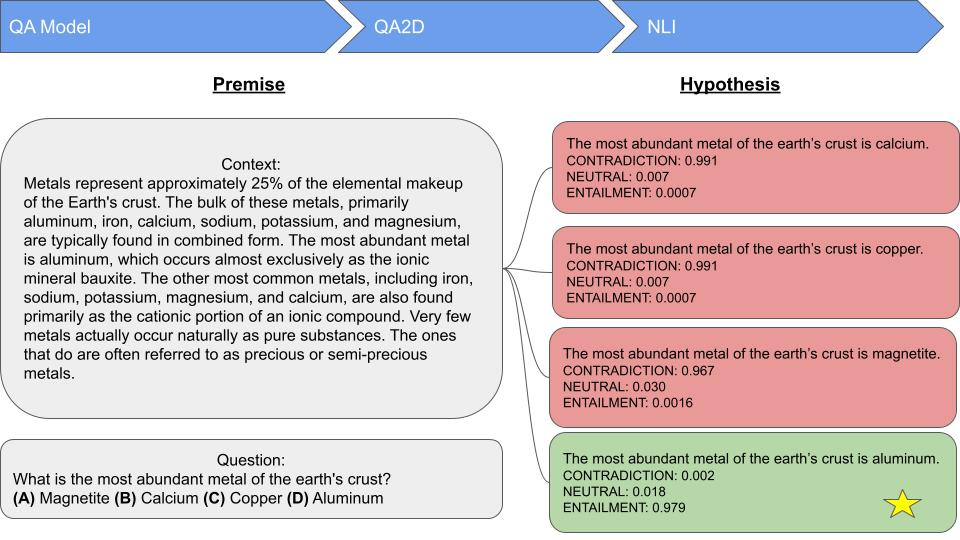
\includegraphics[width=1.0\linewidth]{arch.jpg}
  \caption{A QA model is used to produce answers which are reformulated as hypothesis statements to determine if they are entailed or contradicted by a premise. The answers are ranked by the NLI class scores to select the best answer.}
  \label{fig:architecture}
\end{figure}

These developments are troubling since a verification or self-supporting approach is vulnerable to selecting supporting sources that might be wrong. Since supported or verified answers look more credible, a user might be mislead into uncritically accepting model outputs then they otherwise would be. Even though we could also find sources that wrongly contradict an answer, surfacing sources that contradict an answer might help a user engage critically and help a QA system select the least contradicted answers. Therefore we ask: under NLI-based setups how do contradictions contribute to the performance of question answering (QA) and how is this different from entailment-based systems? By exploring this question, we hope to show why researchers should be critical of the paradigm of verification in NLP systems and why future work utilizing critical and contradicted statements could provide unexplored opportunities for improving NLP systems.

Our work makes the following contributions. We propose a method (Figure \ref{fig:architecture}) that reformulates answers under QA as hypothesis statements which are then used with three-class NLI to rank and select answers. We demonstrate, across 9 multiple choice datasets and 7 extractive QA datasets models, that models which use QA confidence scores as well as both entailment and contradiction scores outperform all other setups. In addition, selecting the least contradicted answer provides a competitive approach to selecting answers that is often on par with or better than entailment-based systems. While this work is in a relatively limited setting, we suggest how leveraging contradictions could help improve QA inference in ways that are not possible with entailment-based systems.
\subsection{Related work}
\textbf{NLI for QA} has been explored by several authors (see the overview in \citet{paramasivam_survey_2021}) showing performance improvements in multiple choice \citep{mishra_looking_2021}, extractive \citep{chen_can_2021}, open domain \citep{harabagiu_methods_2006} and multihop \citep{trivedi_repurposing_2019} settings. These approaches have thus far focused on using entailment as a verification mechanism. \citet{chen_can_2021} find that under selective question answering \citep{kamath_selective_2020} for extractive QA, NLI systems can verify QA systems’ predictions. However, their result is limited to only selecting a top $k$ \% of answers and they do not provide an approach for improving QA systems overall performance nor show what their results would have been like if they incorporated the contradiction signal. \citet{mishra_looking_2021} explores the use of entailment for multiple choice and fact checking settings and finds that not only do NLI models do well at these tasks by themselves but when they are adapted using in-domain data and longer premises they perform even better. Despite this, \citet{mishra_looking_2021} uses a two-class NLI set up (entailed or not entailed) which means there would be no information about the effect of using the contradiction class if this approach was used.

\textbf{Factual consistency} is the only domain that leverages contradictions directly. Factual consistency seeks to ensure that a collection of utterances do not contain contradictions such as unfaithfulness towards a source document (see \citet{li_faithfulness_2022} for an overview). Here approaches to improve faithfulness are still focused on entailment. \citet{laban_summac_2022} proposes a NLI-based method to ensure the consistency of a summary with a source document that incorporates contradiction and neutral scores with entailment scores beating out previous systems. Interestingly, they show that a combination of entailment and contradiction achieves the best results over entailment alone. Similarly, QAFactEval \citep{fabbri_qafacteval_2022} improves on \citet{laban_summac_2022} and maintains the approach of incorporating all NLI class scores. \citet{schuster_stretching_2022} and \citet{hsu_wikicontradiction_2021} develop interesting cases where contradictions are leveraged to identify consistency errors within or across wikipedia articles illustrating the further utility of contradictions. Finally, contradiction detection has surfaced as an important tool in generating dialogues that are consistent with a persona \citep{nie_i_2021, song_generating_2020}. To our knowledge, this is the first work to directly leverage contradictions for QA.
\section{Method}
\subsection{Overview}
The proposed approach is similar to \citet{chen_can_2021} and \citet{mishra_looking_2021} where question answer pairs are turned into declarative statements (QA2D) (see \citet{demszky_transforming_2018}). QA models for each setting are used to produce answers and confidence scores for each answer which are later used to train calibration models. Three-class NLI classification (entailment, neutral, contradiction) is performed on the provided QA contexts (the premises) with the hypotheses produced from the earlier QA2D model. Like \citet{chen_can_2021} a calibration method is used that combines the confidence scores from the QA and NLI models. In the multiple choice setting, answers are selected among a set of alternatives for a given question through ranking by a score produced by the models above. In the extractive QA case, questions are ranked for selective QA \citep{kamath_selective_2020} where a top $k$ number of answers pre-selected by a QA model are selected by how confident the model is in answering a question.
\subsection{QA models}
For the multiple choice setting, we used RoBERTa large \citep{liu_roberta_2019} finetuned on the RACE dataset \citep{lai_race_2017} as well as two DeBERTa v3 \citep{he_debertav3_2021} variants (base and xsmall) finetuned on SciQ \citep{welbl_crowdsourcing_2017}. For the extractive QA setting, we used DistillBERT \citep{sanh_distilbert_2020} and BERT-Large \citep{devlin_bert_2019}) models trained on SQuAD \citep{rajpurkar_squad_2016}. More details on model selection, training, and validation are available in Appendix A. In both cases, answers are selected given a context provided by the dataset and those contexts are used as the premise for NLI.
\subsection{QA2D}
A QA2D model reformulates a question-answer pair to a declarative statement \citep{demszky_transforming_2018}. As noted in \citet{chen_can_2021} and \citet{mishra_looking_2021}, the QA2D reformulation is critical to using NLI models in QA since the proposed answer needs to match the format of NLI. We trained a T5-small model \citep{raffel_exploring_2020} on the dataset proposed by \citet{demszky_transforming_2018} for QA2D since we found almost no noticeable differences in performance in larger models. Unlike \citet{chen_can_2021}, we found that regardless of size, these QA2D models struggled with long questions or questions with complex syntax and would often leave the answer out of the statement. In order to solve this, constrained decoding that required the answer to be in the statement was tried. However, this often produced ungrammatical or nonsensical statements. We settled with the following heuristic to postprocess QA2D outputs: If less than 50\% of the tokens in the answer were in the statement then we appended the answer to the end of the statement. 50\% was used to account for rephrasing the answer or swapping pronouns. While some statements resulted in answer redundancy, this was better than having hypotheses which left out the answer. Future work on QA2D should focus on how these models can be used outside of the domains in the dataset provided by \citet{demszky_transforming_2018}.
\subsection{NLI}
NLI is then used to classify whether the reformulated answer is contradicted, entailed, or neutral w.r.t to a context passage. The whole context was used as \citet{schuster_stretching_2022} and \citet{mishra_looking_2021} demonstrated that long premises still performed adequate though not as well as sentence-length premises. Using the whole context avoids needing to use decontextualization as is required in \citet{chen_can_2021}. We used two DeBERTa-based models \citep{he_deberta_2021} trained on the MNLI dataset \citep{williams-etal-2018-mnli} (called mnli-base and mnli-large) and an ALBERT model \citep{albert} trained on the ANLI dataset in addition to various other NLI datasets (called albert-anli) \citep{nie_adversarial_2020}. After inference, the confidence scores are then used for each class in the procedures below.
\subsection{Calibration models}
Like \citet{kamath_selective_2020} and \citet{chen_can_2021} we developed a set of calibration models in order to do answer ranking. A calibration model is trained on a set of posterior probabilities from downstream models to predict whether an answer is correct. To compare the effect of using different combinations of NLI class confidence scores we trained a logistic regression model on linear combinations of the following features: \textbf{QA} indicates that the QA model confidence score is being used, \textbf{E} indicates the entailment score is used, \textbf{C} indicates the contradiction score is used and \textbf{N} indicates the neutral score. Like \citet{chen_can_2021}, all calibration models are trained on a holdout set of 100 samples from a single domain using logistic regression which predicts, given the confidence scores of the downstream models, whether the answer is correct. A multi-domain calibration approach like in \citet{kamath_selective_2020} was not used since the focus was a minimum experiment to test the viability of leveraging different NLI classifications. To illustrate the characteristics of the calibration models, Appendix D presents a regression analysis for the multiple choice setting.
\subsection{Answer ranking}
Similar to \citet{harabagiu_methods_2006}, answers are ranked based on the highest probability from the calibration model $\sigma$ given a linear combination of the QA or NLI scores given an answer $n \in N$ answer set. When a single feature is used such as NLI class or QA class no calibration is made and $\sigma$ is simply the identity of the confidence score. In the case of contradiction only $\sigma$ is the inverse of the contradiction confidence score, indicating the least contradicted answer is being selected. Formally our approach can be described as:
$$
\underset{N}{\operatorname{argmax}}\:\sigma(QA_n;NLI_n)
$$
For the multiple choice setting we used this for selecting the answer to a given question among a set of alternative answers $N$. We found that using a top $K=4$ approach to extractive QA produced almost the same answer alternatives with slightly different spans so we did not use the alternatives ranking approach with extractive QA. For both the multiple choice and extractive QA settings we ranked answers like in \citet{kamath_selective_2020}, where a top $n$ set of questions at a certain coverage coverage threshold $k$ is selected, resulting in a set of top answers the model is most confident in answering.
\subsection{Datasets}
For both settings, datasets where the context passage is already available were used. For the multiple choice setting a set of 9 datasets were used. Two of those datasets are in-domain for the QA and calibration, RACE and SciQ. For extractive QA 5 of the datasets from the MRQA 2019 task were selected \citep{fisch_mrqa_2019} as well as SQuAD 2.0 \citep{rajpurkar_know_2018} and SQuAD adversarial \citep{jia_adversarial_2017} for a total of 7 extractive QA datasets. The in-domain dataset for the extractive QA model is SQuAD and the dataset used for calibration is Natural Questions since that is what was used by \citet{chen_can_2021}. The only preprocessing done was to remove questions where the context was empty. Appendix B describes full details on the datasets used for evaluation.
\section{Results}
\subsection{Ranking multiple choice}
\begin{table*}[]
\centering
\begin{tabular}{lllllllllll}
\hline
Model & Cosmos & DREAM & MCS & MCS2 & MCT & QASC & RACE & $R_C$ & SciQ & Avg \\ \hline
s-base & 18.46 & 43.80 & 61.99 & 63.71 & 44.76 & 93.41 & 30.97 & 27.39 & 95.28 & 53.30 \\
s-small & 25.46 & 48.26 & 60.28 & 66.04 & 59.76 & 90.60 & 35.56 & 30.62 & 98.09 & 57.18 \\
QA & \textbf{64.22} & \textbf{82.56} & \textbf{89.70} & \textbf{86.98} & {\ul 90.48} & \textbf{98.16} & \textbf{76.93} & \textbf{69.80} & \textbf{97.96} & \textbf{84.08} \\ \hline
E+C & 44.36 & {\ul 80.94} & 85.52 & {\ul 84.99} & \textbf{90.60} & {\ul 96.44} & {\ul 64.29} & {\ul 51.40} & {\ul 92.47} & {\ul 76.77} \\
E & 36.18 & 79.03 & {\ul 86.02} & 79.72 & 89.88 & 95.90 & 62.14 & 49.72 & 91.96 & 74.50 \\
C & {\ul 59.26} & 78.98 & 83.12 & 84.43 & 89.29 & 92.76 & 62.74 & 47.05 & 91.58 & 76.58 \\ \hline
\end{tabular}
\caption{Accuracy scores on NLI-only answer ranking. RoBERTa-RACE is indicated as QA. The best scores are bold and the second best are underlined.}
\label{tab:nli_only_performance}
\end{table*}
\begin{table*}[]
\centering
\begin{tabular}{lllllllllll}
\hline
Model & Cosmos & DREAM & MCS & MCS2 & MCT & QASC & RACE & $R_C$ & SciQ & Avg \\ \hline
s-base & 18.46 & 43.80 & 61.99 & 63.71 & 44.76 & 93.41 & 30.97 & 27.39 & 95.28 & 53.30 \\
s-small & 25.46 & 48.26 & 60.28 & 66.04 & 59.76 & 90.60 & 35.56 & 30.62 & 98.09 & 57.18 \\
QA & 64.22 & 82.56 & 89.70 & 86.98 & 90.48 & 98.16 & 76.93 & \textbf{69.80} & 97.96 & 84.08 \\ \hline
QA+E+C & \textbf{64.72} & \textbf{83.19} & \textbf{90.06} & \textbf{87.59} & \textbf{91.43} & \textbf{98.60} & \textbf{77.53} & \textbf{69.80} & \textbf{98.21} & \textbf{84.57} \\
QA+E & 64.32 & {\ul 82.85} & {\ul 89.92} & {\ul 87.29} & {\ul 91.07} & {\ul 98.49} & {\ul 77.18} & 69.66 & {\ul 98.09} & 84.31 \\
QA+C & {\ul 64.82} & 82.75 & 89.88 & {\ul 87.29} & 90.83 & 98.38 & 77.16 & \textbf{69.80} & {\ul 98.09} & {\ul 84.33} \\ \hline
\end{tabular}
\caption{Accuracy scores on calibrated NLI answer ranking. Calibrations are with the RoBERTa-RACE model (QA). The best scores are bold and the second best are underlined.}
\label{tab:calibrated_performance}
\end{table*}
In tables \ref{tab:nli_only_performance} (NLI only) and \ref{tab:calibrated_performance} (calibrated) we present the accuracy achieved on each of the 9 datasets for the mutiple choice setting. We show results with each QA model and the mnli-large model for NLI (Appendix C shows results for alberta-anli and mnli-base which perform worse but generally reflect the same trends). On the NLI-only results presented in table \ref{tab:nli_only_performance}, the RoBERTA-RACE QA model outperforms other approaches on most datasets except MCTest and the combination of entailment and contradiction tends to do second best. Notably, the SciQ models do much worse than the NLI-only ranking for either class except on in-domain questions for SciQ and the similar QASC dataset. This could possible a result of the RACE domain being more generic than the SciQ domain or the RACE dataset being larger. The results show that an NLI-only approach can be competitive with a robust QA model and better than a more limited QA model. Notably, incorporating the contradiction scores with the entailment scores is better than entailment alone and that selecting the least contradicted answer is quite competitive with selecting the most entailed answer.

The results from the calibration models show that the NLI calibrated models outperform QA only in all cases (they perform the same as RoBERTA-RACE in the in-domain case). The best calibration incorporates QA confidence, entailment, and contradiction (QA+E+C) achieving an average accuracy of 84.57\% over 84.09\% from RoBERTa-RACE. The second best approach is the calibration with contradiction only (84.33\%), however only slightly over entailment only (84.31\%). To inspect these trends further, a correlation analysis in Appendix E is provided on how each NLI class and QA confidence score correlates with the correct answer. Interestingly, other than QA model confidence scores, it is contradiction confidence score that has the strongest correlation with the correct answer further demonstrating the utility of leveraging contradictions.
\subsection{Selective QA}
\begin{table*}[]
\centering
\begin{tabular}{lllllllll}
\hline
 & Database & QA +E+C & QA+C & QA+E & E+C & E & C & QA \\ \hline
20\% & CosmosQA & 77.55 & \textbf{91.12} & 76.88 & 69.18 & 68.34 & 83.25 & {\ul 88.61} \\
 & DREAM & {\ul 98.28} & \textbf{98.77} & {\ul 98.28} & 96.32 & 96.32 & 96.81 & {\ul 98.28} \\
 & MCScript & \textbf{99.82} & 99.46 & \textbf{99.82} & {\ul 99.64} & {\ul 99.64} & 99.46 & \textbf{99.82} \\
 & MCScript-2.0 & {\ul 99.58} & \textbf{99.72} & 99.45 & 99.17 & 99.03 & 97.37 & {\ul 99.58} \\
 & MCTest & \textbf{100} & {\ul 99.40} & \textbf{100} & \textbf{100} & \textbf{100} & {\ul 99.40} & 98.81 \\
 & QASC & \textbf{100} & \textbf{100} & \textbf{100} & \textbf{100} & \textbf{100} & \textbf{100} & \textbf{100} \\
 & RACE & 94.93 & {\ul 96.69} & 94.72 & 92.44 & 92.24 & 90.17 & \textbf{98.24} \\
 & R\_C & 88.73 & {\ul 92.96} & 89.44 & 85.21 & 85.92 & 86.62 & \textbf{93.66} \\
 & SciQ & \textbf{100} & \textbf{100} & \textbf{100} & \textbf{100} & \textbf{100} & \textbf{100} & \textbf{100} \\
 & Avg & 95.43 & \textbf{97.57} & 95.40 & 93.55 & 93.50 & 94.79 & {\ul 97.45} \\ \hline
50\% & CosmosQA & {\ul 80.29} & \textbf{81.70} & 76.94 & 75.80 & 70.64 & 80.63 & 76.47 \\
 & DREAM & 95.10 & \textbf{96.86} & 94.90 & 93.63 & 93.63 & 93.63 & {\ul 96.67} \\
 & MCScript & 98.57 & {\ul 98.64} & 98.28 & 98.00 & 97.93 & 97.14 & \textbf{98.78} \\
 & MCScript-2.0 & 96.40 & \textbf{98.23} & 95.84 & 94.68 & 94.40 & 96.01 & {\ul 98.01} \\
 & MCTest & 99.52 & \textbf{99.76} & 99.52 & 99.05 & 99.05 & {\ul 99.76} & 99.52 \\
 & QASC & \textbf{100} & \textbf{100} & \textbf{100} & {\ul 99.78} & {\ul 99.78} & {\ul 99.78} & \textbf{100} \\
 & RACE & 90.11 & {\ul 92.68} & 89.99 & 87.71 & 87.38 & 85.23 & \textbf{93.88} \\
 & R\_C & 85.11 & 84.83 & {\ul 85.39} & 78.37 & 78.37 & 77.25 & \textbf{87.36} \\
 & SciQ & \textbf{100} & \textbf{100} & \textbf{100} & \textbf{100} & \textbf{100} & 99.74 & \textbf{100} \\
 & Avg & 93.90 & \textbf{94.74} & 93.43 & 91.89 & 91.24 & 92.13 & {\ul 94.52} \\ \hline
\end{tabular}
\caption{Selective QA for the multiple choice with accuracy scores at 20\% and 50\% coverage of the dataset. Calibrations and QA confidence are all from RoBERTa-RACE where RACE is the in-domain dataset.}
\label{tab:selective_mc_qa}
\end{table*}
For selective QA evaluation in both settings, the QA model selects the answer and then we evaluate the top 20\% or 50\% of those answers after sorting them by the approaches we outlined earlier. In the multiple choice setting we do not select the answers for individual questions with the ranking as proposed in the method above since the approach under performed the QA model. Those results are available in Appendix C.
\subsubsection{Selective QA for multiple choice QA}
In table \ref{tab:selective_mc_qa}, the first thing to note is that the QA + C model performs the best on selective QA, achieving best or second best accuracy on almost every dataset for an average of 97.57\% at 20\% coverage and 94.74\% at 50\% coverage over 97.45\% at 20\% coverage and 94.52\% at 50\% coverage achieved by the RoBERTA-RACE QA model. This is especially striking at 50\% coverage where the QA model only does significantly better on the in-domain RACE datasets. The QA+C model is the only model to outperform the QA model ranking by confidence score. The NLI only models can be competitive with the calibrated models. Sorting by the least contradicted achieves good performance and is often better (94.79\% @ 20\% / 92.13\% @ 50\%), than sorting by the most entailed (93.50\% @ 20\% / 91.24\% @ 50\%) or a combination of entailed and contradicted (93.55\% @ 20\% / 91.89\% @ 50\%). These results are inline with our intuition that the less contradicted an answer is the more likely it is correct even in cases where there is uncertainty about its entailment.
\subsubsection{SelectiveQA for extractive QA}
\begin{table*}[]
\centering
\begin{tabular}{lllllllll}
\hline
& Dataset & QA+E+C & QA+E & QA+C & E+C & E & C & QA \\ \hline
20\% & BioASQ & {\ul 85.04} & \textbf{85.06} & 83.10 & 74.22 & 74.22 & 75.47 & 82.99 \\
 & HotpotQA & {\ul 86.62} & \textbf{86.69} & 85.89 & 80.60 & 80.60 & 79.82 & 85.33 \\
 & NaturalQuestions & {\ul 91.84} & 91.68 & \textbf{92.18} & 79.89 & 79.87 & 82.09 & 90.98 \\
 & SQuAD & 98.26 & {\ul 98.76} & 98.17 & 92.37 & 92.48 & 90.88 & \textbf{99.04} \\
 & SQuAD-adv & \textbf{43.99} & {\ul 43.98} & 43.57 & 43.74 & 43.60 & 42.81 & 39.83 \\
 & SQuAD2 & {\ul 37.64} & 37.56 & 36.07 & 37.43 & 37.31 & \textbf{37.68} & 30.52 \\
 & TriviaQA & \textbf{81.33} & 81.21 & 80.36 & 65.53 & 65.25 & 69.13 & 80.68 \\
 & Avg & {\ul 74.96} & \textbf{74.99} & 74.19 & 67.68 & 67.62 & 68.27 & 72.77 \\ \hline
50\% & BioASQ & \textbf{76.13} & {\ul 76.04} & 75.51 & 71.49 & 71.49 & 72.97 & 75.49 \\
 & HotpotQA & \textbf{79.37} & {\ul 79.30} & 78.95 & 77.43 & 77.43 & 77.31 & 78.74 \\
 & NaturalQuestions & \textbf{84.53} & {\ul 84.48} & 83.24 & 74.96 & 74.93 & 78.62 & 82.47 \\
 & SQuAD & {\ul 96.98} & 96.97 & 97.01 & 91.58 & 91.52 & 91.19 & \textbf{97.00} \\
 & SQuAD-adv & 41.80 & 41.16 & 41.49 & {\ul 42.76} & \textbf{42.79} & 42.03 & 40.26 \\
 & SQuAD2 & 29.41 & 28.45 & 28.77 & \textbf{34.43} & 34.14 & {\ul 34.39} & 26.18 \\
 & TriviaQA & 74.30 & \textbf{74.37} & 74.23 & 65.05 & 64.93 & 68.08 & 74.21 \\
 & Avg & \textbf{68.93} & {\ul 68.68} & 68.46 & 65.39 & 65.32 & 66.37 & 67.76 \\ \hline
\end{tabular}
\caption{Selective QA for extractive QA with F1 scores at 20\% and 50\% coverage. Calibrated models and QA use the BERT-large model.}
\label{tab:selective_extractive_qa}
\end{table*}
For the extractive QA setting we present the same analysis in table \ref{tab:selective_extractive_qa}. Similar trends to multiple choice QA are present where calibration with contradiction only, QA + C, has better average F1 scores than the QA model (74.19\% vs 72.77\% at 20\%, 68.46\% vs 67.76\% at 50\%). Of the NLI-only ranking, selecting the least contradicted does best. Although only slightly better than the QA + C, the results show that the QA + E model does best at 20\% coverage and the QA + E + C model does best at 50\% coverage. This indicates that entailment is still an important signal, albeit more powerful when combined with contradiction. Appendix C contains a comparison with the smaller DistillBERT model which shows similar results. Notably with a smaller model QA+E+C does best in all cases and that selecting the least contradicted answer without any calibration does second best at 50\% coverage.
\subsection{Answer Rejection on SQuAD 2.0}
\begin{table*}[t!]
\centering
\begin{tabular}{llllll}
\hline
 & Reject & Accept & Precision & Recall & F1 \\ \hline
QA \textless 50\% & 46.71\% & 86.15\% & 62.81\% & 23.39\% & 34.09\% \\
QA \textless 25\% & 22.29\% & 95.45\% & 71.05\% & 11.16\% & 19.29\% \\
QA  \textless 75\% & 71.22\% & 72.86\% & 56.79\% & 35.66\% & 43.81\% \\
E \textless 5\% & 43.80\% & {\ul 98.74\%} & 94.55\% & 21.93\% & 35.61\% \\
E \textless 25\% & 63.82\% & 96.58\% & 90.33\% & 31.95\% & 47.21\% \\
E \textless 10\% & 52.14\% & 98.02\% & 92.95\% & 26.11\% & 40.77\% \\
E \textless  50\% & \textbf{76.94\%} & 91.52\% & 81.96\% & \textbf{38.52\%} & {\ul 52.41\%} \\
C \textgreater 50\% & 42.78\% & \textbf{99.35\%} & \textbf{97.06\%} & 21.42\% & 35.09\% \\
C \textgreater 25\% & 54.21\% & 98.59\% & {\ul 95.05\%} & 27.15\% & 42.23\% \\
C \textgreater 10\% & 66.88\% & 96.50\% & 90.53\% & 33.49\% & 48.89\% \\
C \textgreater  5\% & {\ul 76.15\%} & 93.23\% & 84.92\% & {\ul 38.13\%} & \textbf{52.63\%} \\ \hline
\end{tabular}
\caption{Rejecting unanswerable questions in SQuAD2.0 (11,873 answers total with 5,945 unanswerable questions). Bold indicates the best score and underlined indicates the second best score.}
\label{tab:rejecting}
\end{table*}
In order to explore how useful contradiction might be in other settings, we evaluated the answer rejection task in SQuAD 2.0 \citep{rajpurkar_know_2018} using our BERT-large model. This task evaluates how well a model does at abstaining from answering a question that is unanswerable. Three setups are used: rejecting answers by QA confidence, by entailment score, and by contradiction score. When selecting by least entailed answers the problem becomes a two-class NLI (entailed v not entailed) which was previously looked at by \citet{chen_can_2021}.

Table \ref{tab:rejecting} shows that the NLI-based setups outperform QA confidence setups in all cases. Interestingly, the difference between rejecting answers that are not entailed and rejecting answers that have been contradicted appears to reflect a precision versus recall trade off. The overall best model (best F1 score) is achieved by rejecting answers where the contradiction score was greater than 5\%, successfully rejecting 76.15\% answers and accepting 93.23\% answerable questions. Rejecting answers if they are not entailed, where E < 50\%, achieves the second best F1 score and illustrates an interesting dynamic. E < 50\% has the best recall (38.52\%), successfully rejecting the most answers, while C > 50\% has the best precision (97.06\%), accepting the most answerable questions. This result shows that if we want to build systems that err on the side of rejecting answers not entailed has an advantage. Conversely, if we want to build systems that are better at rejecting only answers that should be rejected then contradicted is a better strategy. The results highlight the utility of using contradiction confidence scores even if they are low which gives credence to using the contradiction score as a meaningful signal.
\section{Discussion}
While the results above show that contradiction is an important signal for improving performance of QA systems in the settings above, contradiction provides additional unique opportunities for improving NLP systems overall. Contradiction is a particularly important signal because it can improve interpretability. When choosing answers based on the least contradicted answer, we have information about the other answers and why we didn’t select them. Namely, that they were contradicted. Entailment and QA model confidence do not have the same interpretability since all that is known about the other answers is they have a lower entailment or confidence score, they could still be correct or entailed. In addition, we would not know if the unselected alternatives were neutral or contradicted with respect to the premise.

Once an answer is known to be contradicted, that information can be used to try retrieving another answer. In models that support prompting, we can use that contradiction as a hint for another attempt at an answer. Entailment does not lend itself to this iterative refinement of question answering and we suggest that future work on utilizing contradiction should investigate developing inference techniques that take advantage of the contradiction signal.

Contradiction also provides a unique opportunity for open domain QA systems which require retrieving a context containing the answer. Like entailment-based approaches (Harabagiu and Hickl, 2006) we can try selecting the least contradicted passage for a downstream reader. We can also imagine extending the work of \citet{schuster_stretching_2022} where contradiction-based approaches could be used to retrieve passages that would contradict an answer to determine if the proposed answer might be wrong and thereby develop an iterative inference procedure for open domain settings. Retrieved contradicting sources could also be surfaced to a user to help them critically engage with selected answers by the model.

Finally contradicted statements are already being used in a generative setting to improve fact verification systems during train time \citep{wright_generating_2022, pan_zero-shot_2021, saakyan_covid-fact_2021}. Recent work \citep{saunders_self-critiquing_2022} has shown that self-criticism is a powerful technique for improving the quality of NLP systems during inference and we believe generating critical statements for model predictions could help with overall performance, interpretability, and safety by providing outputs with a full picture under which they might be faulty. Future work should assess whether a contradiction-based approaches to improve NLP safety along these lines is an interesting alternative to the current verification-based approaches.
\section{Limitations}
Despite the results above, multiple choice QA and extractive QA with a provided context is a limited setting that doesn’t indicate the results would extend to other popular settings where NLI. Given that \citet{laban_summac_2022} shows similar results that contradiction is an important signal in factual consistency we are hopeful that it would.
\subsection{Context Length and NLI datasets}
Even though there is a greater tendency to use NLI in zero-shot settings \citep{yin_universal_2020}. Domain transfer is a known issue with using NLI models. In particular, NLI datasets tend to focus on textual entailment over short passages such as sentence pairs and performance degrades when using longer passages such as in the datasets we use \citep{mishra_looking_2021}. Even when in-domain datasets are created \citep{chen_can_2021, khot_scitail_2018, mishra_looking_2021}. They tend to focus on data augmentation strategies that produce two-class NLI datasets (entail, not entailed) which wouldn’t give us any contradiction signals. Future work should pick up on producing models capable of performing textual entailment over longer passages and devising methods for generating three-class NLI datasets so that we can determine if contradictions receive the same benefits from those approaches that entailment has. Additionally we saw that albert-anli performed worse than mnli-large and mnli-large performs poorly on some datasets indicating that we still have much more work to do to improve upon NLI in general.
\subsection{Ranking requires alternatives and time}
In the extractive QA setting presented above we did not use ranking answer alternatives like we used for the multiple choice setting due to lack of more diverse outputs. Further work with extractive QA models that produce diverse alternatives is required. Like other textual entailment based systems, this speaks to the computational expense involved in generating and evaluating answer alternatives. If we were to apply our method to an open domain setting where a set of context passages are retrieved, the ranking procedure would require a quadratic evaluation procedure for each context passage against each reformulated answer candidate \citep{schuster_stretching_2022}. Future work should look towards comparison approaches that amortize the computational cost involved in pairwise NLI-based ranking techniques such as investigating NLI-based dense passage retrieval \citep{reimers_sentence-bert_2019}.
\section{Summary}
We have demonstrated that incorporating contradiction is an important signal for multiple choice and extractive QA systems. By proposing a method that reformulates answers as hypothesis statements, the system is able to rank answers and demonstrate that QA model confidence calibrated with entailment and contradiction scores outperform QA models by themselves as a ranking approach in all cases. In addition, models calibrated with contradiction only or simply selecting the least contradicted answers with NLI only provides a competitive approach to selecting answers that is often on par with or better than entailment-only systems. These results show that we should rethink the paradigm of verifying answers with entailment across NLP setups. While this work is in a relatively limited setting, we provide discussion on how leveraging contradictions could help improve open domain QA as well as other NLP tasks at large.
\section{Ethics Statement}
Works addressing NLP safety should be aware of their limitations and be clear about potential harms and misuse of their proposed approaches. Systems that improve safety by verification or support are vulnerable to drawing on untrue and biased sources to justify their outputs. The appearance of credibility given to texts that use citations and appeals to authority means that users should be made aware that the sources they draw on can be wrong. This applies to critical sources as well since a source can provide criticism that is wrong or misleading. However, by presenting contradictions we believe that systems could provide a wider breadth of options for users to engage with critically than models which claim to verify answers by appealing to the authority of a source document.
% Entries for the entire Anthology, followed by custom entries
\bibliography{anthology,custom}
\bibliographystyle{acl_natbib}
\appendix
\section{Training Setup and Reproducibility}
\label{sec:appendix}
\begin{table*}[]
\centering
\begin{tabular}{lll}
\hline
Huggingface & Name \\ \hline
LIAMF-USP/roberta-large-finetuned-RACE & RoBERTa-RACE \\
bert-large-uncased-whole-word-masking-finetuned-squad & BERT-Large \\
distilbert-base-uncased-distilled-squad & DistillBERT \\
ynie/albert-xxlarge-v2-snli\_mnli\_fever\_anli\_R1\_R2\_R3-nli & albert-anli \\
microsoft/deberta-base-mnli & mnli-base \\
microsoft/deberta-v2-xxlarge-mnli & mnli-large \\ \hline
\end{tabular}
\caption{Pretrained models that we used.}
\label{tab:models_trained}
\end{table*}
\begin{table*}[]
\centering
\begin{tabular}{lllll}
\hline
Model & Dataset & Epochs & Score &  \\ \hline
t5-small & \citet{demszky_transforming_2018} & 20 & Rogue1 & 90.73 \\
deberta-v3-xsmall & \citet{welbl_crowdsourcing_2017} & 6 & Accuracy & 93.99 \\
deberta-v3-base & \citet{welbl_crowdsourcing_2017} & 6 & Accuracy & 91.79 \\ \hline
\end{tabular}
\caption{The models we trained for or setups with evaluation scores and number of epochs trained.}
\label{tab:models_trained}
\end{table*}
Table \ref{tab:models_trained} outlines the pretrained models that we used and datasets they are trained on, all of these models are publicly available on the huggingface model hub under the locations listed. Where space doesn't allow RoBERTa-RACE is aliased as RACE.
In addition to several pretrained models used in the setups described earlier, we trained 3 models, a t5-small model on \citet{demszky_transforming_2018} for the QA2D set up where a Rogue1 of 90.73\% is achieved on the validation set, DeBERTa-v3 models (xsmall and base) trained on SciQ \citep{welbl_crowdsourcing_2017} achieving 93.99\% accuracy on the xsmall model and 91.76\% accuracy on the base model. Where space doesn't allow the DeBERTa-v3 models are called s-base and s-small. All models were trained using the huggingface trainer API \citep{wolf_huggingfaces_2020} with an Adam optimizer at a learning rate of 5.60e-05 with weight decay of 0.01. All models and inference were performed on 1 Tesla P100 GPU. More details are available on table \ref{tab:models_trained}.
Full instructions on reproducibility as well as trained models are provided in the publicly available code including directions to weights and biases to inspect the training runs, full parameter set, and evaluations suites which will be available upon publication.
\section{Dataset Details}
\label{sec:appendix}
The tables (Table \ref{tab:mc_qa_datasets} and Table \ref{tab:extractive_qa_datasets}) below outline the datasets used . Additional details such as train size and preprocessing steps are available in the references provided. When space doesn't allow CosmosQA is aliased to Cosmos, MCScript to MCS, MCScript-2.0 to MCS2, MCTest to MCT, and RACE-C to $R_C$. As mentioned previously the only preprocessing step used was to filter out questions where no context passage is provided. Finally, validation splits are used in the CosmosQA and QASC case since context passages or gold answers are not made available so readers should be aware of this when reading results on those datasets.
\begin{table*}[t!]
\centering
\begin{tabular}{llll}
\hline
Dataset & Split & Size & Reference \\ \hline
CosmosQA & validation & 2985 & \citet{huang_cosmos_2019} \\
DREAM & test & 2041 & \citet{sun_dream_2019} \\
MCScript & test & 2797 & \citet{ostermann_mcscript_2018} \\
MCScript-2.0 & test & 3610 & \citet{ostermann_mcscript20_2019}) \\
MCTest & test & 840 & \citet{richardson_mctest_2013} \\
QASC & validation & 926 & \citet{khot_qasc_2020} \\
RACE & test & 4934 & \citet{lai_race_2017} \\
RACE-C & test & 712 & \citet{liang_new_2019}) \\
SciQ & test & 884 & \citet{welbl_crowdsourcing_2017} \\ \hline
\end{tabular}
\caption{Datasets used for the multiple choice setting including split used and sample size. Validation splits were used in the case of CosmosQA since the test split is not publicly available and QASC since context passages or gold answers are not available.}
\label{tab:mc_qa_datasets}
\end{table*}
\begin{table*}[]
\centering
\begin{tabular}{lll}
\hline
Dataset & Size & Reference \\ \hline
BioASQ & 1504 & \citet{fisch_mrqa_2019} \\
TriviaQA & 7785 &  \\
HotpotQA & 5901 &  \\
SQuAD & 10506 &  \\
Natural Questions & 12836 &  \\
SQuAD2 & 11871 & \citet{rajpurkar_know_2018} \\
SQuAD-adv & 5347 & \cite{jia_adversarial_2017} \\ \hline
\end{tabular}
\caption{Extractive QA datasets used. Validation sets are used on the SQuAD2.0 and SQuAD adversarial datasets and MRQA 2019 dev sets are used for the MRQA 2019 sets.}
\label{tab:extractive_qa_datasets}
\end{table*}
\section{Model size and approach performance analysis}
\label{sec:appendix}
\begin{table*}[]
\centering
\begin{tabular}{llllllllllll}
\hline
Model & Cosmos & Dream & MCS & MCS2 & MCT & QASC & RACE & $R_C$ & SciQ & Avg \\ \hline
SciQ-base & 18.46 & 43.80 & 61.99 & 63.71 & 44.76 & 93.41 & 30.97 & 27.39 & 95.28 & 53.31 \\
SciQ-small &  25.46 & 48.26 & 60.28 & 66.04 & 59.76 & 90.60 & 35.56 & 30.62 & 98.09 & 57.19 \\
RACE & 64.22 & 82.56 & 89.70 & 86.98 & 90.48 & 98.16 & 76.93 & 69.80 & 97.96 & 84.09 \\ \hline
mnli-base \\ 
 QA + E + C & 64.32 & 82.66 & 89.63 & 87.01 & 90.71 & 98.27 & 76.95 & 69.80 & 98.09 & 84.16 \\
  QA + E & 64.25 & 82.66 & 89.63 & 86.98 & 90.71 & 98.27 & 76.95 & 69.80 & 97.96 & 84.14 \\
  QA + C & 64.29 & 82.56 & 89.63 & 87.01 & 90.60 & 98.16 & 76.93 & 69.80 & 97.96 & 84.1 \\
  E + C & 33.03 & 62.27 & 76.76 & 72.11 & 68.57 & 92.66 & 45.16 & 34.41 & 88.01 & 63.66 \\
  E & 27.81 & 62.47 & 79.37 & 71.94 & 68.81 & 92.66 & 43.48 & 34.41 & 88.01 & 63.22 \\
  C & 43.45 & 59.19 & 70.18 & 69.97 & 67.50 & 81.86 & 41.81 & 32.58 & 87.37 & 61.55 \\ \hline
 albert-anli \\ 
QA + E + C & 64.19 & 82.56 & 89.70 & 87.06 & 90.48 & 98.16 & 76.93 & 69.80 & 97.96 & 84.09 \\
  QA + E & 64.19 & 82.56 & 89.70 & 87.06 & 90.60 & 98.16 & 76.93 & 69.80 & 97.96 & 84.11 \\
  QA + C & 64.22 & 82.56 & 89.70 & 86.98 & 90.48 & 98.16 & 76.93 & 69.80 & 97.96 & 84.09 \\
  E + C & 35.71 & 68.20 & 79.55 & 73.88 & 77.50 & 91.79 & 49.05 & 39.47 & 90.82 & 67.33 \\
  E & 33.67 & 68.35 & 79.91 & 73.19 & 77.38 & 91.90 & 49.07 & 39.19 & 90.94 & 67.07 \\
  C & 45.16 & 63.74 & 73.58 & 72.71 & 73.33 & 77.86 & 46.34 & 38.20 & 87.24 & 64.24 \\ \hline
\end{tabular}
\caption{Accuracy scores in the multiple choice setting for various NLI models used. Calibration was with the RoBERTA-RACE model.}
\label{tab:cross_mc_performance}
\end{table*}
In order to help understand how the results presented above differ with model size or approach we have presented the following supplemental tables. Table \ref{tab:cross_mc_performance} shows differences in performance between mnli-base, mnli-large, and albert-anli. Table \ref{tab:selective_ranking} shows selective QA accuracies in the multiple choice setting where answer selection is done through ranking before we rank answers for selective QA. Selective QA on extractive QA using DistillBERT (table \ref{tab:selective_distillbert}) shows that QA+E+C does best in all cases and contradiction only does second best at 50\% coverage.
\begin{table*}[]
\centering
\begin{tabular}{lllllllll}
\hline
 & Dataset & QA+E+C & QA+E & QA+C & E+C & E & C & QA \\ \hline
20\% & CosmosQA & 77.55 & 67.17 & {\ul 83.25} & 20.10 & 27.47 & 67.50 & \textbf{88.61} \\
 & DREAM & \textbf{98.28} & 96.32 & {\ul 96.81} & 81.13 & 91.91 & 93.87 & \textbf{98.28} \\
 & MCScript & \textbf{99.82} & \textbf{99.64} & {\ul 99.46} & 93.02 & {\ul 98.93} & 96.96 & \textbf{99.82} \\
 & MCScript-2.0 & \textbf{99.58} & {\ul 99.03} & 97.37 & 92.24 & 97.37 & 95.01 & \textbf{99.58} \\
 & MCTest & \textbf{100} & \textbf{100} & {\ul 99.40} & 85.12 & 97.02 & 97.02 & 98.81 \\
 & QASC & \textbf{100} & \textbf{100} & \textbf{100} & 97.30 & \textbf{100} & {\ul 99.46} & \textbf{100} \\
 & RACE & {\ul 94.93} & 92.13 & 90.17 & 62.73 & 76.71 & 75.05 & \textbf{98.24} \\
 & RACE-C & {\ul 88.73} & 85.21 & 86.62 & 71.13 & 74.65 & 69.01 & \textbf{93.66} \\
 & SciQ & \textbf{100} & \textbf{100} & \textbf{100} & 82.05 & 100 & 96.15 & \textbf{100} \\
 & Avg & {\ul 95.43} & 93.28 & {\ul 94.79} & 76.09 & 84.90 & 87.78 & \textbf{97.45} \\ \hline
50\% & CosmosQA & {\ul 80.29} & 70.78 & \textbf{80.70} & 32.17 & 34.72 & 64.88 & 76.47 \\
 & DREAM & {\ul 95.10} & 93.63 & 93.63 & 85.20 & 89.41 & 88.33 & \textbf{96.67} \\
 & MCScript & \textbf{98.57} & {\ul 97.85} & 97.14 & 94.71 & 95.99 & 92.70 & \textbf{98.78} \\
 & MCScript-2.0 & {\ul 96.40} & 94.46 & {\ul 96.07} & 91.02 & 91.75 & 91.69 & \textbf{98.01} \\
 & MCTest & \textbf{99.52} & {\ul 98.81} & \textbf{99.76} & 91.43 & 95.24 & 96.19 & \textbf{99.52} \\
 & QASC & \textbf{100} & \textbf{99.78} & \textbf{99.78} & 98.27 & {\ul 98.70} & 98.49 & \textbf{100} \\
 & RACE & {\ul 90.11} & 87.22 & 85.23 & 67.89 & 71.70 & 68.18 & \textbf{93.88} \\
 & RACE-C & {\ul 85.11} & 78.09 & 77.25 & 66.57 & 66.85 & 55.06 & \textbf{87.36} \\
 & SciQ & \textbf{100} & \textbf{100} & \textbf{99.74} & 89.03 & 96.43 & 96.43 & \textbf{100} \\
 & Avg & {\ul 93.90} & 91.18 & 92.14 & 79.59 & 82.31 & 83.55 & \textbf{94.52} \\ \hline
\end{tabular}
\caption{Selective QA accuracies in the multiple choice setting where answer selection is done through ranking before we rank answers for selective QA.}
\label{tab:selective_ranking}
\end{table*}
\begin{table*}[]
\centering
\begin{tabular}{lllllllll}
\hline
 & Dataset & QA+E+C & QA+E & QA+C & E+C & E & C & QA \\ \hline
20\% & BioASQ & 70.97 & 70.41 & 71.55 & {\ul 74.07} & {\ul 74.07} & \textbf{74.34} & 68.99 \\
 & HotpotQA & \textbf{73.44} & {\ul 73.08} & 70.88 & 71.59 & 71.51 & 70.41 & 69.41 \\
 & NaturalQuestions & \textbf{85.59} & 85.29 & {\ul 85.45} & 78.46 & 78.46 & 80.53 & 83.27 \\
 & SQuAD & 96.22 & {\ul 96.45} & 95.77 & 83.15 & 83.09 & 81.37 & \textbf{97.15} \\
 & SQuAD-adv & {\ul 40.39} & 39.75 & 39.49 & 40.07 & 39.56 & \textbf{40.59} & 31.98 \\
 & SQuAD2 & 35.46 & 35.24 & 33.64 & {\ul 36.36} & 36.13 & \textbf{36.66} & 25.95 \\
 & TriviaQA & \textbf{64.96} & {\ul 64.68} & 64.55 & 52.67 & 52.09 & 52.56 & 63.98 \\
 & Avg & \textbf{66.72} & {\ul 66.41} & 65.90 & 62.34 & 62.13 & 62.35 & 62.96 \\ \hline
50\% & BioASQ & {\ul 65.96} & 65.92 & 64.37 & 63.53 & 63.53 & \textbf{66.95} & 64.79 \\
 & HotpotQA & 64.42 & 64.21 & 63.65 & 65.88 & {\ul 65.85} & \textbf{66.91} & 62.81 \\
 & NaturalQuestions & {\ul 72.28} & 71.99 & 70.82 & 67.54 & 67.51 & \textbf{74.18} & 69.95 \\
 & SQuAD & {\ul 92.56} & \textbf{92.57} & 92.34 & 81.86 & 82.21 & 80.95 & 92.54 \\
 & SQuAD-adv & 33.69 & 32.90 & 33.45 & \textbf{38.74} & 38.22 & {\ul 38.52} & 31.89 \\
 & SQuAD2 & 26.68 & 25.70 & 26.00 & \textbf{32.95} & 32.61 & {\ul 32.83} & 23.52 \\
 & TriviaQA & {\ul 58.40} & \textbf{58.41} & 58.25 & 51.43 & 51.18 & 52.99 & 58.25 \\
 & Avg & \textbf{59.14} & 58.81 & 58.41 & 57.42 & 57.30 & {\ul 59.05} & 57.68 \\ \hline
\end{tabular}
\caption{SelectiveQA on extractive QA using DistillBERT. Note that QA+E+C does best in all cases and contradiction only does second best at 50\% coverage.}
\label{tab:selective_distillbert}
\end{table*}
\section{Regression Analysis}
\begin{table*}[]
\centering
\begin{tabular}{lllllll}
\hline
QA Model & NLI Model & Combination & Confidence & Entailment & Contradiction & Acc \\ \hline
SciQ & mnli-base & QA + C & 4.13 &  & -1.06 & 0.99 \\
 &  & QA + E & 3.90 & 1.37 &  & 0.99 \\
 &  & QA + E + C & 3.83 & 1.22 & -0.76 & 0.99 \\
 &  & E + C &  & 2.56 & -1.47 & 0.86 \\
 & mnli-large & QA + C & 3.98 &  & -1.32 & 0.99 \\
 &  & QA + E & 3.78 & 1.55 &  & 0.99 \\
 &  & QA + E + C & 3.65 & 1.31 & -0.97 & 0.99 \\
 &  & E + C &  & 2.63 & -1.72 & 0.91 \\
RACE & mnli-base & QA + C & 3.04 &  & -0.15 & 0.89 \\
 &  & QA + E & 3.03 & 0.27 &  & 0.89 \\
 &  & QA + E + C & 3.02 & 0.26 & -0.14 & 0.89 \\
 &  & E + C &  & 0.73 & -0.46 & 0.75 \\
 & mnli-large & QA + C & 2.97 & 0.00 & -0.81 & 0.89 \\
 &  & QA + E & 2.91 & 0.98 &  & 0.89 \\
 &  & QA + E + C & 2.85 & 0.92 & -0.75 & 0.89 \\
 &  & E + C &  & 1.76 & -1.12 & 0.78 \\ \hline
\end{tabular}
\caption{Regression analysis for each mnli-based nli model with each QA model used calibration with logistic regression multiple choice settings. Accuracy is the evaluation metric used.}
\label{tab:regression_analysis}
\end{table*}
Table \ref{tab:regression_analysis} shows a supplemental regression analysis for each calibration model used in the multiple choice settings. The results indicate that as the MNLI model gets larger the calibration model uses its NLI confidence scores more. Importantly entailment coefficients are stronger than contradiction coefficients in all cases and this should be kept in mind when considering the results presented in this paper.
\section{Correlation Analysis}
\begin{table*}[]
\centering
\begin{tabular}{llllllll}
\hline
 &  & Contradiction &  & Entailment &  & Neutral &  \\ \hline
Dataset & QA & Score & Class & Score & Class & Score & Class \\
CosmosQA & \textbf{0.53} & {\ul -0.34} & -0.17 & 0.05 & -0.01 & 0.21 & 0.16 \\
DREAM & \textbf{0.72} & {\ul -0.57} & -0.35 & 0.54 & 0.50 & -0.11 & -0.13 \\
MCScript & \textbf{0.80} & {\ul -0.59} & -0.42 & {\ul 0.59} & 0.50 & -0.04 & -0.08 \\
MCScript2 & \textbf{0.77} & {\ul -0.50} & -0.32 & 0.41 & 0.37 & -0.04 & -0.05 \\
MCTest & \textbf{0.73} & -0.65 & -0.47 & 0.64 & {\ul 0.69} & -0.20 & -0.15 \\
QASC & {\ul 0.57} & -0.54 & -0.28 & 0.55 & \textbf{0.67} & -0.50 & -0.26 \\
RACE & \textbf{0.65} & {\ul -0.37} & -0.20 & 0.35 & 0.34 & -0.11 & -0.11 \\
RACE-C & \textbf{0.59} & -0.24 & -0.13 & 0.18 & {\ul 0.25} & -0.09 & -0.11 \\
SciQ & \textbf{0.75} & {\ul -0.69} & -0.47 & 0.68 & 0.67 & -0.42 & -0.19 \\ \hline
\end{tabular}
\caption{Correlation analysis (Spearman rank correlation) per dataset in the multiple choice setting. RoBERTa-RACE is used for the QA scores.}
\label{tab:per_dataset_correlation}
\end{table*}
\begin{table*}[]
\centering
\begin{tabular}{llllll}
\hline
 &  & Contradiction & Entailment & Neutral & QA \\ \hline
multiple choice & Score & \textbf{-0.47} & 0.37 & -0.06 & 0.71 \\
 & Class & -0.28 & \textbf{0.38} & -0.06 &  \\
extractive QA & Score & -0.16 & \textbf{0.31} & -0.12 & 0.19 \\
 & Class & -0.15 & \textbf{0.39} & -0.29 &  \\ \hline
\end{tabular}
\caption{Correlation analysis (Spearman rank correlation) in the multiple choice and extractive QA settings. RoBERTa-RACE is the QA model used for multiple choice QA scores and BERT-large is used for the extractive QA scores.}
\label{tab:correlation}
\end{table*}
Since we are using the NLI and QA model scores to construct the setups above, we’d like to know how these factors correlate with the correct answer. Table \ref{tab:correlation} shows how each NLI class correlates both by score and by actual classification (score > 50\%) as compared against QA model confidence score. The multiple choice analysis shows answers from the RoBERTa-RACE model and the extractive QA analysis shows answers from the BERT-large model trained on SQuAD. The correlation analysis presents Spearman rank correlations. What we see is that in the multiple choice setting the confidence score has a strong correlation with the correct answer which makes sense given the confidence score is a softmax over the multiple choice classes. Extractive QA confidence scores have a much weaker correlation and tend to have less correlation than entailment has with the correct answer. Despite the results presented above, contradiction only has a notable correlation with the correct answer when the score is used rather than the classification. This is another proof point of our approach of using confidence scores for NLI rather than classifications. Interestingly in the extractive QA case the neutral class is more negatively correlated when selecting for contradiction when using classification. Our conjecture would be that in the extractive QA case we don’t have much to compare against. When looking at the per dataset correlations for the multiple choice setting (Table \ref{tab:per_dataset_correlation}) we see that in most cases, other than the QA confidence scores, the contradiction scores have the strongest correlations with the correct answer out of any NLI class and neutral, as we would expect, tends to have very weak correlations. We do not present the per dataset correlation for extractive QA as they are very weak, which we again hypothesize comes from having no answers to compare with.
\end{document}